\documentclass[12pt, a4paper]{article}

\usepackage[margin=2.5cm]{geometry}
\usepackage{graphicx}
\usepackage{hyperref}
\usepackage{booktabs}
\usepackage{array}
\usepackage{parskip}
\usepackage{titlesec}
\usepackage{xcolor}
\usepackage{fontenc}
\usepackage{inputenc}
\usepackage{tikz}
\usepackage{float}
\usetikzlibrary{shapes.geometric, arrows.meta, positioning, fit, backgrounds, calc}

\hypersetup{
    colorlinks=true,
    linkcolor=blue,
    urlcolor=blue,
    citecolor=blue
}

\titleformat{\section}{\large\bfseries}{}{0em}{}[\titlerule]
\titleformat{\subsection}{\normalsize\bfseries}{}{0em}{}

% Define colors for diagrams
\definecolor{xenpurple}{RGB}{88, 44, 131}
\definecolor{qubesblue}{RGB}{41, 128, 185}
\definecolor{securegreen}{RGB}{39, 174, 96}
\definecolor{warnorange}{RGB}{230, 126, 34}
\definecolor{lightgray}{RGB}{245, 245, 245}

\begin{document}

%---------------------------------------------------------------
% COVER PAGE
%---------------------------------------------------------------
\begin{titlepage}
    \centering
    \vspace*{1cm}

    \includegraphics[width=0.25\textwidth]{gsoc_logo.png}\\[0.4cm]
    {\large\textbf{Google Summer of Code 2026}}\\[0.3cm]
    {\large @}\\[0.8cm]

    \includegraphics[width=0.35\textwidth]{images.png}\\[0.3cm]
    {\large\textbf{QUBES OS}}\\
    {\small\textit{A Reasonably Secure Operating System}}\\[1.5cm]

    {\LARGE\textbf{Proposal}}\\[0.4cm]
    {\LARGE\textbf{Secure Boot Support for Qubes OS}}\\[2cm]

    {\large\textbf{Harshit Bhalani}}\\[0.2cm]
    {\normalsize March 29, 2026}

    \vfill
\end{titlepage}

%---------------------------------------------------------------
% TABLE OF CONTENTS
%---------------------------------------------------------------
\tableofcontents
\newpage

%---------------------------------------------------------------
% APPLICANT TABLE
%---------------------------------------------------------------
\begin{table}[h]
\centering
\begin{tabular}{>{\bfseries}p{4cm} p{9cm}}
\toprule
Applicant    & Harshit Bhalani \\
Email        & \href{mailto:harshitbhalani6@gmail.com}{harshitbhalani6@gmail.com} \\
GitHub       & \href{https://github.com/Harshit6-b}{github.com/Harshit6-b} \\
Mentor       & Marek Marczykowski-G\'{o}recki \\
Organization & Invisible Things Lab / Qubes OS \\
Size         & 175 hours \\
Time Zone    & UTC+05:30 (IST) \\
\bottomrule
\end{tabular}
\end{table}

%---------------------------------------------------------------
% 1. INTRODUCTION
%---------------------------------------------------------------
\section{Introduction}

Qubes OS builds its entire security model on hardware-enforced isolation. Yet this isolation only begins \textit{after} the bootloader runs; the boot chain itself is unsigned and unverified. An attacker with physical access, a compromised firmware update, or a supply-chain compromise can silently replace Xen, the Dom0 kernel, or boot parameters before Qubes initialises. UEFI Secure Boot is precisely the mechanism designed to close this gap.

\begin{figure}[H]
\centering
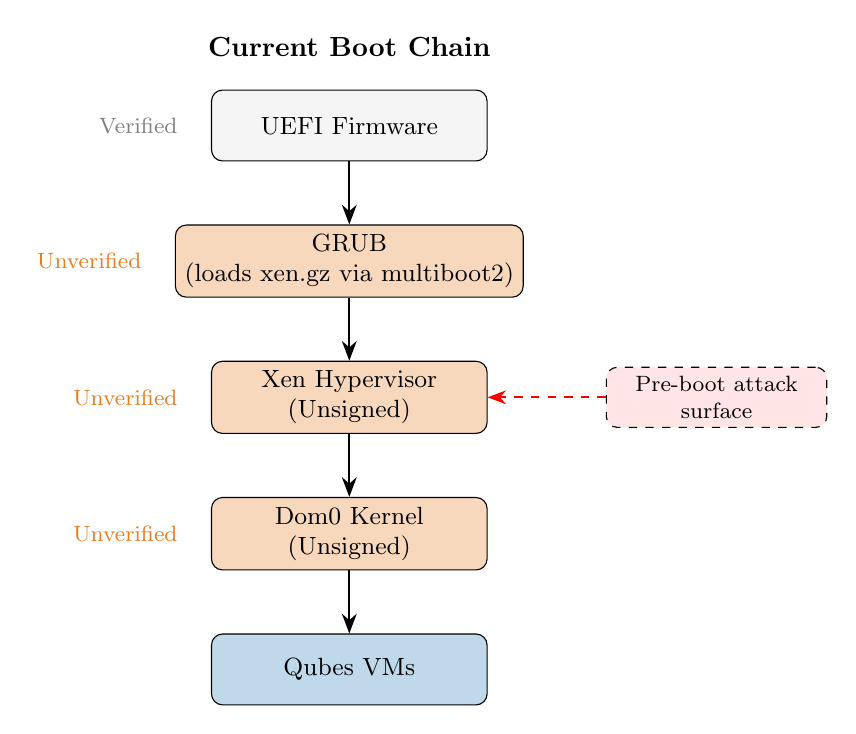
\begin{tikzpicture}[
    node distance=0.8cm,
    every node/.style={font=\small},
    block/.style={rectangle, draw, rounded corners, minimum width=3.5cm, minimum height=0.9cm, align=center},
    attack/.style={rectangle, draw, dashed, fill=red!10, rounded corners, minimum width=2.8cm, minimum height=0.7cm, align=center, font=\footnotesize},
    arrow/.style={-{Stealth[length=2.5mm]}, thick}
]

% Current insecure boot chain
\node[block, fill=lightgray] (uefi) {UEFI Firmware};
\node[block, fill=warnorange!30, below=of uefi] (grub) {GRUB\\(loads xen.gz via multiboot2)};
\node[block, fill=warnorange!30, below=of grub] (xen) {Xen Hypervisor\\(Unsigned)};
\node[block, fill=warnorange!30, below=of xen] (dom0) {Dom0 Kernel\\(Unsigned)};
\node[block, fill=qubesblue!30, below=of dom0] (qubes) {Qubes VMs};

% Attack surface note
\node[attack, right=1.5cm of xen] (atk) {Pre-boot attack\\surface};

% Arrows
\draw[arrow] (uefi) -- (grub);
\draw[arrow] (grub) -- (xen);
\draw[arrow] (xen) -- (dom0);
\draw[arrow] (dom0) -- (qubes);

\draw[-{Stealth}, dashed, red, thick] (atk) -- (xen);

% Labels
\node[left=0.3cm of uefi, font=\footnotesize, text=gray] {Verified};
\node[left=0.3cm of grub, font=\footnotesize, text=warnorange] {Unverified};
\node[left=0.3cm of xen, font=\footnotesize, text=warnorange] {Unverified};
\node[left=0.3cm of dom0, font=\footnotesize, text=warnorange] {Unverified};

% Title
\node[above=0.3cm of uefi, font=\bfseries] {Current Boot Chain};

\end{tikzpicture}
\caption{Current Qubes boot chain without Secure Boot. GRUB loads Xen via multiboot2, then Xen loads Dom0. None of these components are cryptographically verified.}
\label{fig:current-boot}
\end{figure}

Since recent releases, Xen supports a ``unified EFI boot'' model in which Xen, the Dom0 kernel, initramfs, and boot parameters are bundled into a single PE/COFF binary called a Unified Kernel Image (UKI) that can be signed as one unit and verified by UEFI firmware before any code executes. Qubes R4.3 will ship with pre-built unified \texttt{xen.efi} binaries via the \href{https://github.com/QubesOS/qubes-vmm-xen-unified}{\texttt{qubes-vmm-xen-unified}} repository, but the user-facing tooling to sign these binaries, generate keys, handle updates, and provide fallback recovery does not yet exist.

A Qubes user who wants Secure Boot today faces a fully manual process: no tooling to sign the UKI with user-generated keys, no guidance on key generation and enrollment, no integration with the update mechanism (meaning a kernel update silently breaks Secure Boot), and no fallback path for recovery. This project builds that integration end-to-end, extending the existing \texttt{qubes-vmm-xen-unified} infrastructure with signing, key management, and update hooks.

See \href{https://github.com/QubesOS/qubes-issues/issues/4371}{issue \#4371} and \href{https://github.com/QubesOS/qubes-issues/issues/8206}{issue \#8206} for the upstream discussion.

%---------------------------------------------------------------
% 2. PROJECT GOALS
%---------------------------------------------------------------
\section{Project Goals}

\subsection*{Committed Deliverables for the GSoC Term}

\begin{enumerate}
    \item \textbf{UKI Signing Tool (\texttt{qubes-uki-sign}):} Signs the pre-built unified \texttt{xen.efi} from \texttt{qubes-vmm-xen-unified} with user-generated keys, configurable via \texttt{/etc/qubes/secureboot.conf}

    \item \textbf{Key Management (\texttt{qubes-sb-keygen}):} Generates a PK/KEK/db key hierarchy with configurable key parameters, produces EFI authenticated variable files (\texttt{.auth}), and provides step-by-step enrollment instructions

    \item \textbf{Update Integration:} A post-transaction RPM hook that automatically re-signs the UKI whenever \texttt{qubes-vmm-xen-unified} or Dom0 kernel packages are updated, with \texttt{qubes-pecheck} verification before installation

    \item \textbf{Fallback Recovery:} A fallback UKI (\texttt{qubes-fallback.efi}) built from a last-known-good snapshot, registered as a lower-priority UEFI boot entry, with \texttt{qubes-uki-promote-fallback} command

    \item \textbf{Documentation:} Complete coverage of key generation, signing workflow, enrollment, update integration, and recovery procedures
\end{enumerate}

\textbf{Starter Task (Pre-GSoC):} Fix two \texttt{qubes-pecheck} false positives identified during analysis of real-world EFI binaries. These patches will be submitted during community bonding.

\subsection*{Explicitly Out of Scope}

\begin{itemize}
    \item Microsoft CA signing path (blocked upstream by Xen's missing SBAT support and NX\_COMPAT issues)
    \item TPM-based remote attestation or PCR-based sealing
    \item Multi-kernel support beyond the active Dom0 kernel
\end{itemize}

%---------------------------------------------------------------
% 3. IMPLEMENTATION
%---------------------------------------------------------------
\section{Implementation Details}

\subsection{Secure Boot Architecture Overview}

The core solution transforms the vulnerable boot chain into a cryptographically verified sequence. UEFI firmware validates the UKI signature against enrolled keys before transferring control to Xen, which then loads the embedded Dom0 kernel.

\begin{figure}[H]
\centering
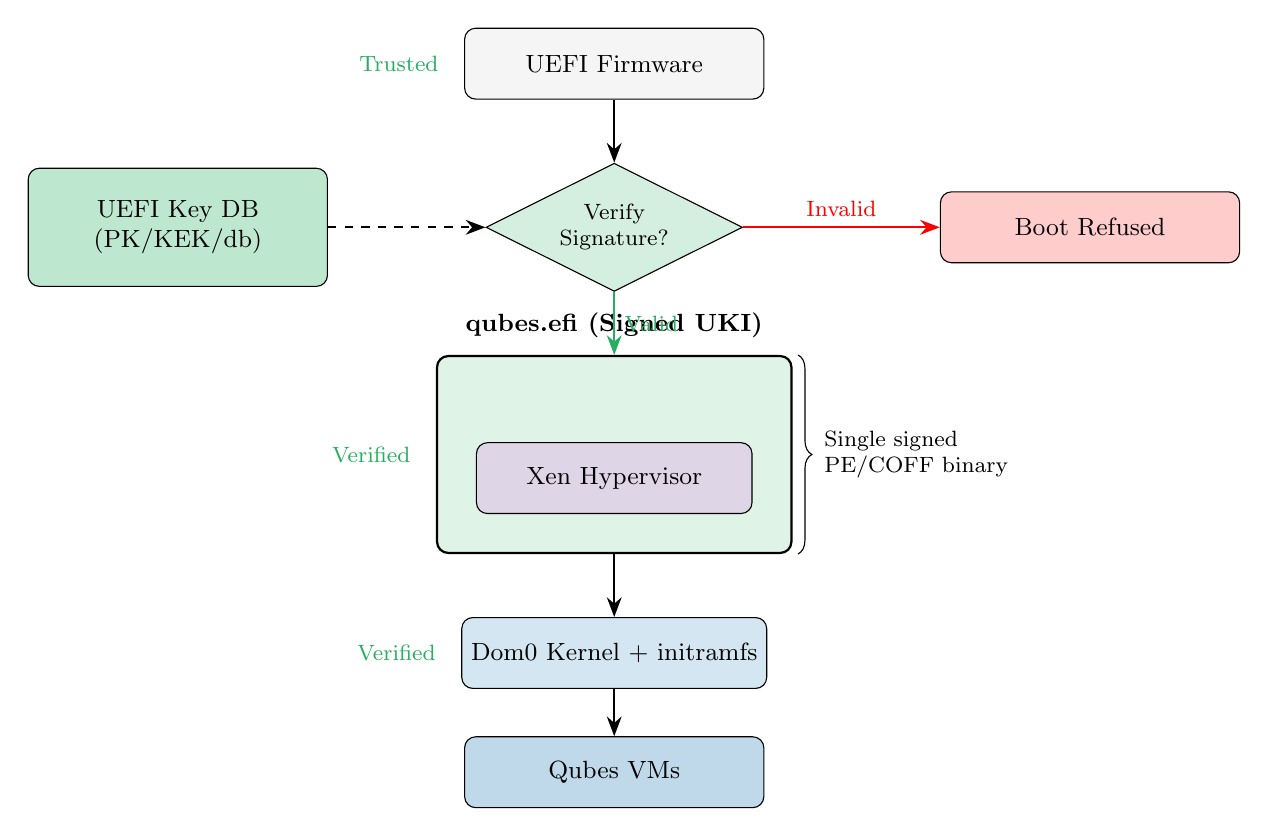
\begin{tikzpicture}[
    node distance=0.6cm and 1.5cm,
    every node/.style={font=\small},
    block/.style={rectangle, draw, rounded corners, minimum width=3.8cm, minimum height=0.9cm, align=center},
    verify/.style={diamond, draw, aspect=2, fill=securegreen!20, minimum width=2cm, align=center, font=\footnotesize},
    arrow/.style={-{Stealth[length=2.5mm]}, thick},
    signed/.style={rectangle, draw, thick, fill=securegreen!15, rounded corners}
]

% Boot sequence
\node[block, fill=lightgray] (uefi) {UEFI Firmware};
\node[verify, below=0.8cm of uefi] (check) {Verify\\Signature?};
\node[signed, below=0.8cm of check, minimum width=4.5cm, minimum height=2.5cm] (uki) {};
\node[above=0.1cm] at (uki.north) {\textbf{qubes.efi (Signed UKI)}};
\node[block, fill=xenpurple!20, minimum width=3.5cm] at ([yshift=-0.3cm]uki.center) (xen) {Xen Hypervisor};
\node[block, fill=qubesblue!20, below=0.8cm of uki] (dom0) {Dom0 Kernel + initramfs};
\node[block, fill=qubesblue!30, below=of dom0] (qubes) {Qubes VMs};

% Failed path
\node[block, fill=red!20, right=2.5cm of check] (fail) {Boot Refused};

% Key database
\node[block, fill=securegreen!30, left=2cm of check, minimum height=1.5cm] (keys) {UEFI Key DB\\(PK/KEK/db)};

% Arrows
\draw[arrow] (uefi) -- (check);
\draw[arrow, securegreen] (check) -- node[right, font=\footnotesize] {Valid} (uki);
\draw[arrow, red] (check) -- node[above, font=\footnotesize] {Invalid} (fail);
\draw[arrow] (uki) -- (dom0);
\draw[arrow] (dom0) -- (qubes);
\draw[arrow, dashed] (keys) -- (check);

% Signature indicator
\draw[decorate, decoration={brace, amplitude=5pt, raise=2pt}]
    (uki.north east) -- (uki.south east)
    node[midway, right=8pt, font=\footnotesize, align=left] {Single signed\\PE/COFF binary};

% Labels
\node[left=0.2cm of uefi, font=\footnotesize, text=securegreen] {Trusted};
\node[left=0.2cm of uki, font=\footnotesize, text=securegreen] {Verified};
\node[left=0.2cm of dom0, font=\footnotesize, text=securegreen] {Verified};

\end{tikzpicture}
\caption{Secure Boot architecture with UKI. UEFI firmware verifies the signed UKI against enrolled keys before executing any Qubes code.}
\label{fig:secure-boot}
\end{figure}

\subsection{UKI Structure and Assembly}

The \texttt{qubes-vmm-xen-unified} package produces a unified \texttt{xen.efi} binary by embedding Dom0 kernel, initramfs, and boot parameters into the existing Xen EFI binary. The assembly process uses \texttt{objcopy --add-section} to append sections after Xen's \texttt{.pad} section, preserving the original PE structure:

\begin{table}[H]
\centering
\begin{tabular}{>{\ttfamily}p{2.5cm} p{7cm} p{3cm}}
\toprule
\normalfont\textbf{Section} & \textbf{Contents} & \textbf{Source} \\
\midrule
(Xen native)  & Xen hypervisor code and data sections & xen.efi (base) \\
.pad         & Alignment padding (assembly point) & xen.efi (base) \\
.cmdline     & Xen and kernel command-line & Embedded \\
.initrd      & initramfs + microcode blobs & Embedded \\
.linux       & Dom0 kernel (vmlinuz) & Embedded \\
\bottomrule
\end{tabular}
\end{table}

\begin{figure}[H]
\centering
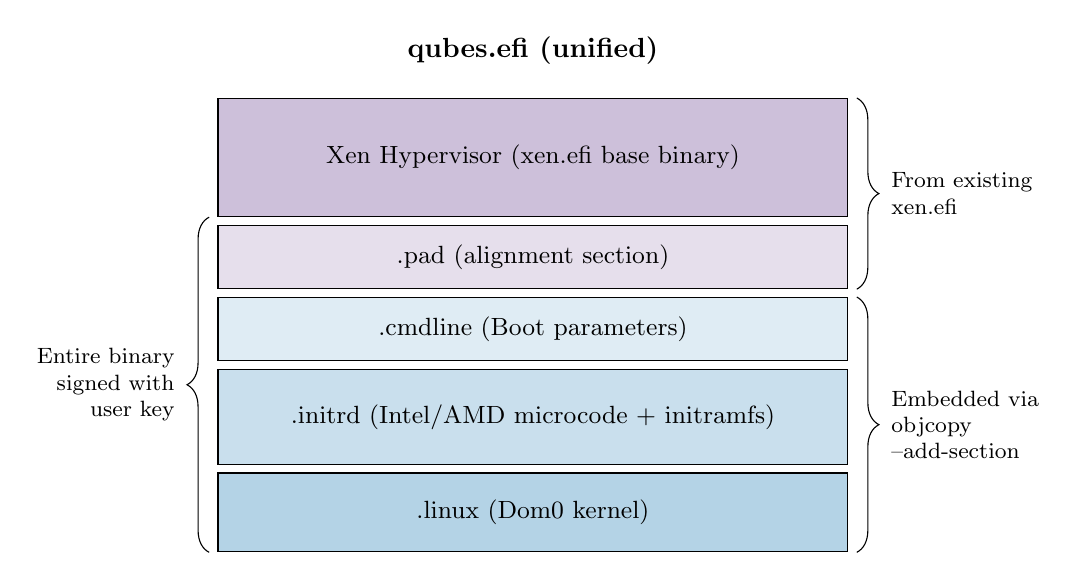
\begin{tikzpicture}[
    every node/.style={font=\small},
    section/.style={rectangle, draw, minimum width=8cm, minimum height=0.8cm, align=center},
    label/.style={font=\footnotesize, text=gray}
]

% Base xen.efi
\node[section, fill=xenpurple!30, minimum height=1.5cm] (xen) {Xen Hypervisor (xen.efi base binary)};
\node[section, fill=xenpurple!15, below=0.1cm of xen] (pad) {.pad (alignment section)};

% Embedded sections
\node[section, fill=qubesblue!15, below=0.1cm of pad] (cmdline) {.cmdline (Boot parameters)};
\node[section, fill=qubesblue!25, below=0.1cm of cmdline, minimum height=1.2cm] (initrd) {.initrd (Intel/AMD microcode + initramfs)};
\node[section, fill=qubesblue!35, below=0.1cm of initrd, minimum height=1cm] (linux) {.linux (Dom0 kernel)};

% Braces
\draw[decorate, decoration={brace, amplitude=8pt, raise=3pt}]
    (xen.north east) -- (pad.south east)
    node[midway, right=12pt, font=\footnotesize, align=left] {From existing\\xen.efi};

\draw[decorate, decoration={brace, amplitude=8pt, raise=3pt}]
    (cmdline.north east) -- (linux.south east)
    node[midway, right=12pt, font=\footnotesize, align=left] {Embedded via\\objcopy\\--add-section};

% Signature brace
\draw[decorate, decoration={brace, amplitude=8pt, mirror, raise=3pt}]
    (xen.south west) -- (linux.south west)
    node[midway, left=12pt, font=\footnotesize, align=right] {Entire binary\\signed with\\user key};

% File name
\node[above=0.3cm of xen, font=\bfseries] {qubes.efi (unified)};

\end{tikzpicture}
\caption{UKI structure. The unified binary embeds Dom0 kernel and initramfs into the existing Xen EFI binary, which is then signed as a single unit.}
\label{fig:uki-structure}
\end{figure}

This project does not re-implement UKI assembly; \texttt{qubes-vmm-xen-unified} already handles that. The \texttt{qubes-uki-sign} tool takes the pre-built unified binary and signs it with the user's db key using \texttt{sbsign}. Configuration is read from \texttt{/etc/qubes/secureboot.conf}, specifying key paths and signing parameters.

\subsection{Key Hierarchy and Management}

UEFI Secure Boot uses a hierarchical key structure. This project implements user-controlled keys, giving Qubes users full sovereignty over their boot chain without depending on Microsoft or any third-party CA.

\begin{figure}[H]
\centering
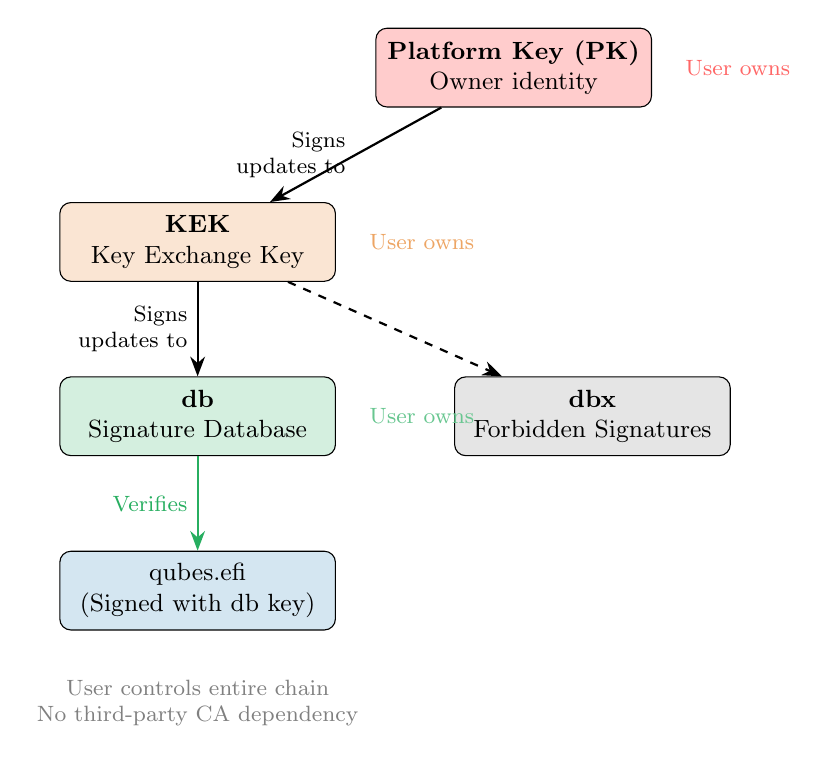
\begin{tikzpicture}[
    node distance=1.2cm,
    every node/.style={font=\small},
    key/.style={rectangle, draw, rounded corners, minimum width=3.5cm, minimum height=1cm, align=center},
    arrow/.style={-{Stealth[length=2.5mm]}, thick}
]

% Key hierarchy
\node[key, fill=red!20] (pk) {\textbf{Platform Key (PK)}\\Owner identity};
\node[key, fill=warnorange!20, below left=1.2cm and 0.5cm of pk] (kek) {\textbf{KEK}\\Key Exchange Key};
\node[key, fill=securegreen!20, below=1.2cm of kek] (db) {\textbf{db}\\Signature Database};
\node[key, fill=gray!20, right=1.5cm of db] (dbx) {\textbf{dbx}\\Forbidden Signatures};

% UKI connection
\node[key, fill=qubesblue!20, below=1.2cm of db] (uki) {qubes.efi\\(Signed with db key)};

% Arrows showing hierarchy
\draw[arrow] (pk) -- node[left, font=\footnotesize, align=right] {Signs\\updates to} (kek);
\draw[arrow] (kek) -- node[left, font=\footnotesize, align=right] {Signs\\updates to} (db);
\draw[arrow, dashed] (kek) -- (dbx);
\draw[arrow, securegreen] (db) -- node[left, font=\footnotesize] {Verifies} (uki);

% Ownership indicator
\node[right=0.3cm of pk, font=\footnotesize, text=red!60] {User owns};
\node[right=0.3cm of kek, font=\footnotesize, text=warnorange!70] {User owns};
\node[right=0.3cm of db, font=\footnotesize, text=securegreen!70] {User owns};

% Description
\node[below=0.5cm of uki, font=\footnotesize, text=gray, align=center] {User controls entire chain\\No third-party CA dependency};

\end{tikzpicture}
\caption{UEFI Secure Boot key hierarchy. The user owns all keys, ensuring complete control over the trusted boot chain.}
\label{fig:key-hierarchy}
\end{figure}

The \texttt{qubes-sb-keygen} subcommand generates the full PK/KEK/db hierarchy with configurable key parameters (RSA-2048 to RSA-4096, defaulting to RSA-4096). It produces:
\begin{itemize}
    \item EFI signature list (\texttt{.esl}) files for each key
    \item Authenticated variable update (\texttt{.auth}) files for enrollment
    \item Step-by-step enrollment instructions for both \texttt{efi-updatevar} and \texttt{mokutil}
\end{itemize}

\subsection{Update Hook and Atomic Replacement}

The update hook is a post-transaction RPM scriptlet that triggers on updates to \texttt{qubes-vmm-xen-unified} or \texttt{kernel-qubes-dom0}.

\begin{figure}[H]
\centering
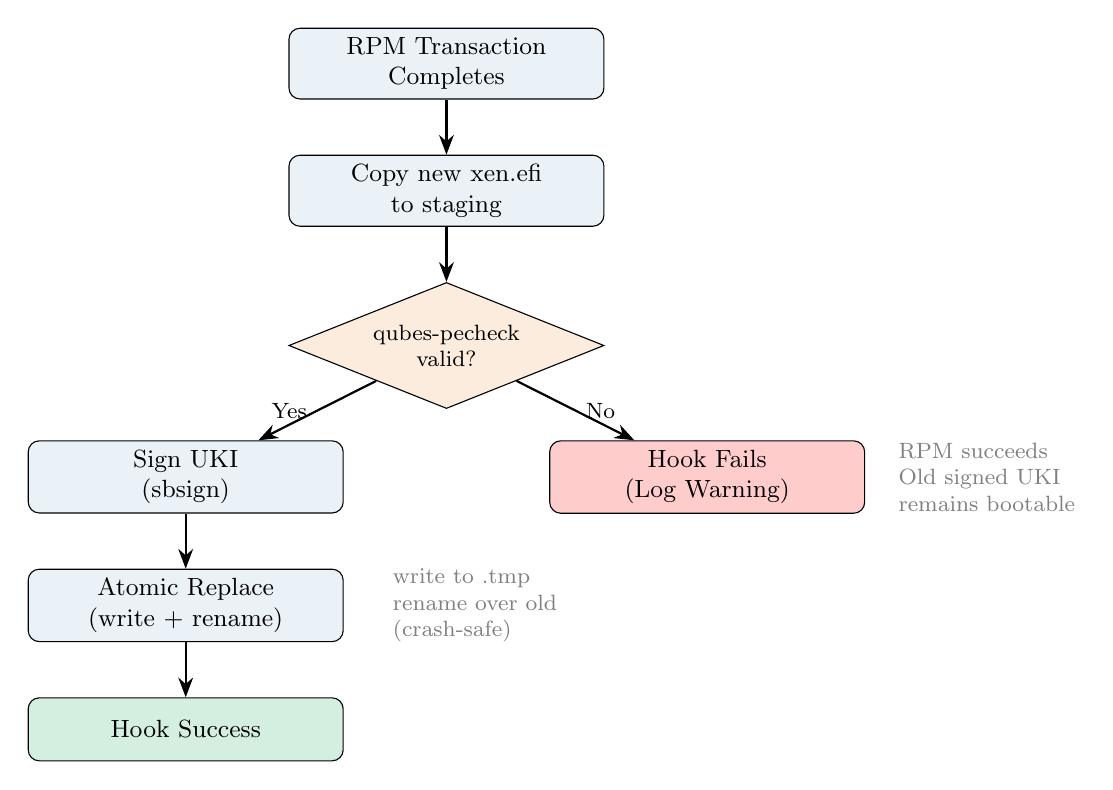
\begin{tikzpicture}[
    node distance=0.7cm,
    every node/.style={font=\small},
    process/.style={rectangle, draw, rounded corners, minimum width=4cm, minimum height=0.8cm, align=center, fill=qubesblue!10},
    decision/.style={diamond, draw, aspect=2.5, fill=warnorange!15, align=center, font=\footnotesize},
    arrow/.style={-{Stealth[length=2.5mm]}, thick}
]

% Process flow
\node[process] (update) {RPM Transaction\\Completes};
\node[process, below=of update] (copy) {Copy new xen.efi\\to staging};
\node[decision, below=of copy] (pecheck) {qubes-pecheck\\valid?};
\node[process, below left=0.8cm and 0.3cm of pecheck] (sign) {Sign UKI\\(sbsign)};
\node[process, below=of sign] (atomic) {Atomic Replace\\(write + rename)};
\node[process, below=of atomic, fill=securegreen!20] (done) {Hook Success};

% Failure path
\node[process, below right=0.8cm and 0.3cm of pecheck, fill=red!20] (fail) {Hook Fails\\(Log Warning)};

% Arrows
\draw[arrow] (update) -- (copy);
\draw[arrow] (copy) -- (pecheck);
\draw[arrow] (pecheck) -- node[left, font=\footnotesize] {Yes} (sign);
\draw[arrow] (pecheck) -- node[right, font=\footnotesize] {No} (fail);
\draw[arrow] (sign) -- (atomic);
\draw[arrow] (atomic) -- (done);

% Note on failure
\node[right=0.3cm of fail, font=\footnotesize, text=gray, align=left] {RPM succeeds\\Old signed UKI\\remains bootable};

% Note on atomic
\node[right=0.5cm of atomic, font=\footnotesize, text=gray, align=left] {write to .tmp\\rename over old\\(crash-safe)};

\end{tikzpicture}
\caption{Update hook workflow. The hook runs post-transaction; RPM package installation always succeeds. Signing failure leaves the previous UKI intact.}
\label{fig:update-hook}
\end{figure}

\textbf{Critical design decision:} The hook runs \textit{after} the RPM transaction completes, not as a blocking pre-transaction check. This ensures package updates never fail due to signing issues. If signing fails, the hook logs a warning but the old signed UKI remains in place, keeping the system bootable. The user can manually re-run signing after resolving the issue (e.g., providing the correct key passphrase).

The atomic replacement writes the new signed UKI to a temporary file, then renames it over the active boot entry. If replacement is interrupted (power loss, crash), the previous signed UKI remains in place.

\subsection{Fallback and Recovery}

The fallback UKI (\texttt{qubes-fallback.efi}) represents a last-known-good state, providing recovery when the primary UKI fails.

\begin{figure}[H]
\centering
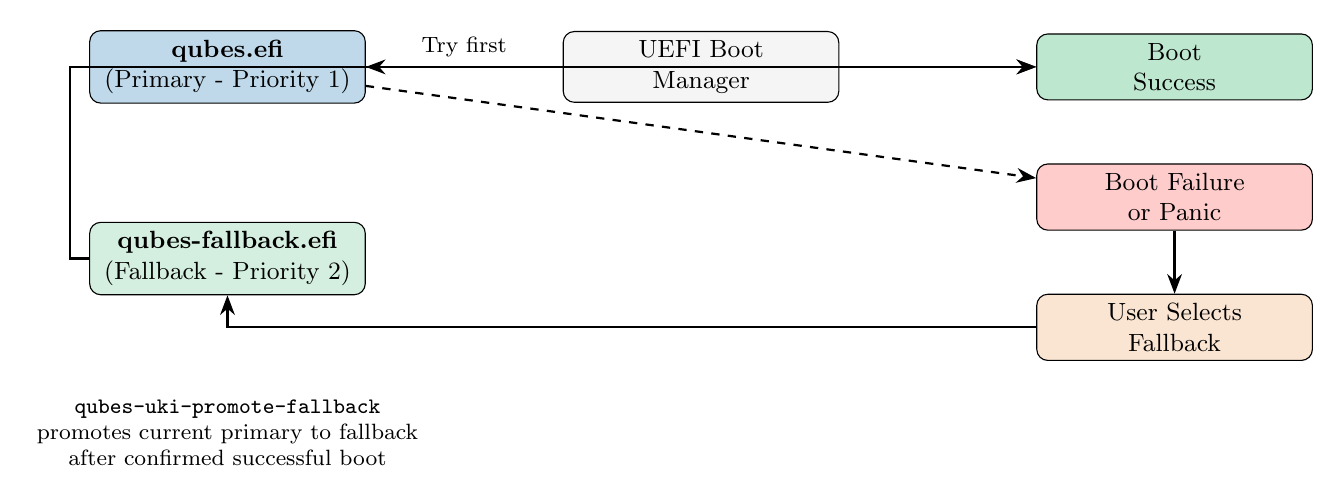
\begin{tikzpicture}[
    node distance=0.8cm and 2cm,
    every node/.style={font=\small},
    block/.style={rectangle, draw, rounded corners, minimum width=3.5cm, minimum height=0.8cm, align=center},
    arrow/.style={-{Stealth[length=2.5mm]}, thick}
]

% Boot entries
\node[block, fill=qubesblue!30] (primary) {\textbf{qubes.efi}\\(Primary - Priority 1)};
\node[block, fill=securegreen!20, below=1.5cm of primary] (fallback) {\textbf{qubes-fallback.efi}\\(Fallback - Priority 2)};

% Decision
\node[block, fill=lightgray, right=2.5cm of primary] (uefi) {UEFI Boot\\Manager};

% Outcomes
\node[block, fill=securegreen!30, right=2.5cm of uefi] (success) {Boot\\Success};
\node[block, fill=red!20, below=of success] (panic) {Boot Failure\\or Panic};
\node[block, fill=warnorange!20, below=of panic] (manual) {User Selects\\Fallback};

% Arrows
\draw[arrow] (uefi) -- node[above, font=\footnotesize] {Try first} (primary);
\draw[arrow] (primary) -- (success);
\draw[arrow, dashed] (primary) -- (panic);
\draw[arrow] (panic) -- (manual);
\draw[arrow] (manual) -| (fallback);
\draw[arrow] (fallback) -- ++(-2,0) |- (success);

% Promotion
\node[below=1.2cm of fallback, font=\footnotesize, align=center] (promote) {\texttt{qubes-uki-promote-fallback}\\promotes current primary to fallback\\after confirmed successful boot};

\end{tikzpicture}
\caption{Fallback recovery flow. Users can recover from a bad update by selecting the fallback entry from the UEFI boot menu.}
\label{fig:fallback}
\end{figure}

The fallback is deliberately not auto-updated. It only changes when the user explicitly runs \texttt{qubes-uki-promote-fallback} after confirming the primary UKI boots correctly.

\textbf{Troubleshooting limitation:} UKI bundles prevent runtime modification of boot parameters. If the primary UKI boots but Qubes misbehaves, users cannot add debug flags at the GRUB prompt as they could with traditional boot. The fallback addresses catastrophic failures (signature mismatch, kernel panic), but for parameter debugging, users must either: (1) rebuild a debug UKI with modified parameters and sign it, or (2) temporarily disable Secure Boot. The documentation will cover both workflows.

\subsection{qubes-pecheck Fixes}

As part of my starter task, I ran \texttt{qubes-pecheck} against real-world EFI and UKI binaries. Two false positives are directly relevant:

\textbf{False positive 1: \texttt{SizeOfRawData < VirtualSize}}\\
The current check rejects Microsoft EFI binaries with this condition. However, this is valid per the PE/COFF specification when a section contains BSS-style zero-filled data. The fix allows this case and only fails when \texttt{SizeOfRawData} is zero and \texttt{VirtualSize} is non-zero.

\textbf{False positive 2: \texttt{.linux} section flagged as non-executable}\\
The \texttt{.linux} section carries the Dom0 kernel blob, which is data loaded by Xen, not code that executes at the PE level. The fix distinguishes between executable sections and well-known UKI data sections (\texttt{.linux}, \texttt{.initrd}, \texttt{.cmdline}).

Both patches will be submitted during community bonding.

%---------------------------------------------------------------
% 4. CHALLENGES AND MITIGATIONS
%---------------------------------------------------------------
\section{Challenges and Mitigations}

\subsection*{Challenge 1: UEFI Variable Space Exhaustion}

\textbf{Risk:} Some firmware implementations have severely limited NVRAM space for UEFI variables. Enrolling multiple keys or creating multiple boot entries can exhaust this space, potentially bricking the system.

\textbf{Mitigation:}
\begin{itemize}
    \item Check available NVRAM space before enrollment operations
    \item Use compact \texttt{.esl} format rather than verbose alternatives
    \item Provide clear warnings and dry-run mode for enrollment
    \item Document recovery procedures for exhausted NVRAM
\end{itemize}

\subsection*{Challenge 2: OEM-Locked Firmware (No Custom PK)}

\textbf{Risk:} Some OEM firmware does not allow replacing the Platform Key, preventing direct enrollment of user keys into the db.

\textbf{Mitigation:}
\begin{itemize}
    \item Support the MOK (Machine Owner Key) path via \texttt{mokutil} and Shim
    \item Detect OEM-locked firmware and guide user to appropriate enrollment method
    \item Document which path applies to common hardware vendors
\end{itemize}

\subsection*{Challenge 3: Signing Key Security}

\textbf{Risk:} If the user's signing key is compromised, an attacker can sign malicious UKIs that will pass Secure Boot verification.

\textbf{Mitigation:}
\begin{itemize}
    \item Document secure key storage practices (encrypted partition, hardware token)
    \item Support keys stored on external media for offline signing workflows
    \item Recommend key rotation procedures in documentation
\end{itemize}

\subsection*{Challenge 4: Testing Environment Limitations}

\textbf{Risk:} QEMU/OVMF may not perfectly replicate real firmware behavior, especially edge cases in NVRAM handling and boot entry management.

\textbf{Mitigation:}
\begin{itemize}
    \item Use QEMU/OVMF for rapid iteration during development
    \item Validate critical paths on real hardware before midterm
    \item Document tested hardware configurations
\end{itemize}

%---------------------------------------------------------------
% 5. TIMELINE
%---------------------------------------------------------------
\section{Timeline and Project Plan}

\begin{table}[H]
\centering
\small
\begin{tabular}{p{2.8cm} p{3cm} p{7.5cm}}
\toprule
\textbf{Date / Period} & \textbf{Phase} & \textbf{Detailed Sub-Tasks} \\
\midrule
May 1 -- May 26 & Community Bonding &
Finalise \texttt{secureboot.conf} schema with Marek. Set up QEMU + OVMF test environment. Submit \texttt{qubes-pecheck} patches. Review \texttt{qubes-vmm-xen-unified} build scripts. \\
\midrule
Week 1--2 \newline (May 27 -- June 9) & Signing Core &
Implement \texttt{qubes-uki-sign} wrapper around \texttt{sbsign}. Parse \texttt{secureboot.conf}. Unit tests with real unified binaries in QEMU/OVMF. \\
\midrule
Week 3--4 \newline (June 10 -- June 23) & Key Generation &
Implement \texttt{qubes-sb-keygen}: configurable RSA key generation, \texttt{.esl}/\texttt{.auth} production. Test full sign-and-enroll cycle in OVMF. \\
\midrule
Week 5--6 \newline (June 24 -- July 7) & Update Hook &
Implement RPM post-transaction hook. Add \texttt{qubes-pecheck} verification. Implement atomic replacement. Test full update cycle. \\
\midrule
\textbf{July 8--11} & \textbf{Midterm} &
\textbf{Deliverable:} Signing + key generation + update hook, end-to-end tested in QEMU with real \texttt{qubes-vmm-xen-unified} binaries. \\
\midrule
Week 7--8 \newline (July 12 -- July 25) & Fallback UKI &
Implement fallback generation and boot entry registration via \texttt{efibootmgr}. Implement \texttt{qubes-uki-promote-fallback}. Test recovery path. \\
\midrule
Week 9--10 \newline (July 26 -- Aug 8) & Edge Cases \& UX &
MOK path via \texttt{mokutil}. Handle: missing microcode, NVRAM exhaustion, failed \texttt{sbsign}. Begin user documentation. \\
\midrule
Week 11--12 \newline (Aug 9 -- Aug 22) & Docs \& Review &
Complete user and developer documentation. Extended testing. Incorporate Marek's review feedback. \\
\midrule
Aug 22 -- Sep 1 & Buffer &
Bug fixes, cleanup, final PR polish. \\
\bottomrule
\end{tabular}
\end{table}

\subsection*{Visual Timeline}

\begin{figure}[H]
\centering
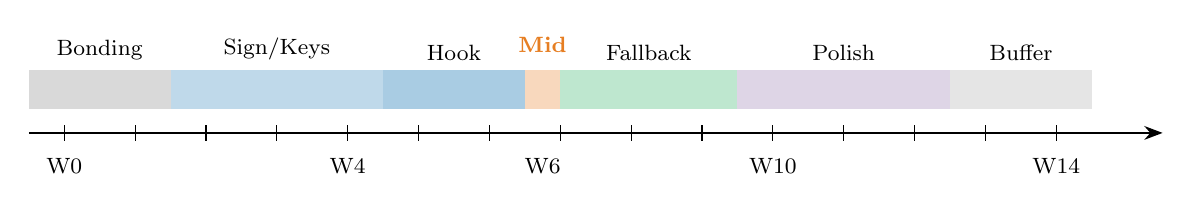
\begin{tikzpicture}[
    x=0.9cm,
    every node/.style={font=\footnotesize}
]

% Timeline base
\draw[thick, -{Stealth}] (0,0) -- (16,0);

% Week markers
\foreach \x in {0,1,...,14} {
    \draw (\x+0.5, 0.1) -- (\x+0.5, -0.1);
}

% Phase blocks
\fill[gray!30] (0,0.3) rectangle (2,0.8);
\fill[qubesblue!30] (2,0.3) rectangle (5,0.8);
\fill[qubesblue!40] (5,0.3) rectangle (7,0.8);
\fill[warnorange!30] (7,0.3) rectangle (7.5,0.8);
\fill[securegreen!30] (7.5,0.3) rectangle (10,0.8);
\fill[xenpurple!20] (10,0.3) rectangle (13,0.8);
\fill[gray!20] (13,0.3) rectangle (15,0.8);

% Labels
\node[above] at (1,0.8) {Bonding};
\node[above] at (3.5,0.8) {Sign/Keys};
\node[above] at (6,0.8) {Hook};
\node[above, text=warnorange] at (7.25,0.9) {\textbf{Mid}};
\node[above] at (8.75,0.8) {Fallback};
\node[above] at (11.5,0.8) {Polish};
\node[above] at (14,0.8) {Buffer};

% Week labels
\node[below] at (0.5,-0.2) {W0};
\node[below] at (4.5,-0.2) {W4};
\node[below] at (7.25,-0.2) {W6};
\node[below] at (10.5,-0.2) {W10};
\node[below] at (14.5,-0.2) {W14};

\end{tikzpicture}
\caption{GSoC timeline overview. Midterm deliverable at Week 6 includes working signing, key generation, and update integration.}
\label{fig:timeline}
\end{figure}

\subsection*{Exam Disclosure}

My end-semester exams at VJTI fall in May. Exact dates have not yet been released. I will communicate specific dates to Marek as soon as they are available and front-load community bonding tasks around the exam window.

\subsection*{Communication Plan}

\begin{itemize}
    \item \textbf{Weekly:} Formal progress update to \texttt{qubes-devel} every Monday covering completed work, next steps, and blockers
    \item \textbf{Ongoing:} Open PR/branch maintained throughout for incremental review. Responsive on Matrix and email within 24 hours
\end{itemize}

%---------------------------------------------------------------
% 6. ABOUT ME
%---------------------------------------------------------------
\section{About Me \& Commitments}

\subsection*{Basic Information}

\begin{itemize}
    \item \textbf{Name:} Harshit Bhalani
    \item \textbf{University:} Veermata Jijabai Technological Institute (VJTI), Mumbai, India
    \item \textbf{Major:} B.Tech in Electronics and Telecommunication Engineering (Second Year), Minor in Data Science
    \item \textbf{CGPA:} 9.02 / 10
    \item \textbf{GitHub:} \href{https://github.com/Harshit6-b}{github.com/Harshit6-b}
    \item \textbf{Email:} \href{mailto:harshitbhalani6@gmail.com}{harshitbhalani6@gmail.com}
    \item \textbf{Mailing lists:} Subscribed to \texttt{qubes-devel}
    \item \textbf{Core Stack:} Python, Bash, Verilog, C
\end{itemize}

\subsection*{Technical Background}

I am a second-year Electronics and Telecommunication Engineering student at VJTI Mumbai and a Core SY Member of the Society of Robotics and Automation (SRA-VJTI). My background is in digital hardware (RTL design in Verilog, FPGA development on Xilinx Artix-7, and embedded systems), but I work comfortably in Python and Bash, which are the primary languages for this project.

I came to this project through genuine study of the Qubes boot stack. I watched the Qubes OS Summit talks and the Xen Winter Meetup 2025, read through issues \#4371 and \#8206, and studied the UEFI specification before reaching out to Marek. Building an understanding of the full UEFI boot sequence (SEC$\to$PEI$\to$DXE$\to$BDS$\to$TSL$\to$RT), the Secure Boot key hierarchy (PK/KEK/db/dbx), Shim/MOK, and PE/COFF format required significant self-directed effort.

\subsection*{Prior Contributions to Qubes OS}

\textbf{qubes-core-agent-linux PR \#644:} Open, under review by Marek.

Fixes a race condition in \texttt{qubes-firewall} (issues \#3735/\#10643). Root cause: \texttt{sd\_notify('READY=1')} fires before initialisation completes, causing SIGHUP to interrupt \texttt{qdb.read()} mid-protocol. An initial retry-loop fix was rejected because interrupting \texttt{qdb.read()} after sending a request desynchronises the QubesDB protocol. The approved approach uses \texttt{signal.pthread\_sigmask} to block SIGHUP/SIGTERM during all qdb operations.

\textbf{qubes-pecheck starter task:} Analysis complete, patches in progress.

Ran \texttt{qubes-pecheck} against Microsoft, Ubuntu, openSUSE, and Arch UKI binaries. Identified two false positives described in the Implementation section. Patches are a community bonding goal.

\subsection*{Organization Specific Questions}

\begin{itemize}
    \item \textbf{Are you comfortable working independently under a supervisor several thousand miles away?}

    Yes. My entire interaction with Marek on PR \#644 has been asynchronous across time zones without difficulty. I plan to use weekly \texttt{qubes-devel} updates and an open PR branch to maintain full visibility.

    \item \textbf{If your native language is not English, are you comfortable working closely with a supervisor whose native language is English?}

    My native languages are Marathi, Hindi, and Gujarati, but I communicate in English fluently and have no concerns about technical communication with Marek.

    \item \textbf{Are you submitting proposals to other organizations?}

    No. Qubes OS is my only application.
\end{itemize}

\subsection*{Commitments}

My university examinations conclude in May. I will treat this as a full-time commitment, dedicating a minimum of 40 hours per week throughout the GSoC coding period. This proposal has been reviewed by a senior member of SRA-VJTI before submission.

%---------------------------------------------------------------
% 7. REFERENCES
%---------------------------------------------------------------
\section{References}

\begin{itemize}
    \item Qubes Secure Boot Discussion: \href{https://github.com/QubesOS/qubes-issues/issues/4371}{Issue \#4371}
    \item Xen UKI Support: \href{https://github.com/QubesOS/qubes-issues/issues/8206}{Issue \#8206}
    \item Qubes Unified Xen: \href{https://github.com/QubesOS/qubes-vmm-xen-unified}{qubes-vmm-xen-unified repository}
    \item UEFI Specification: \href{https://uefi.org/specifications}{uefi.org/specifications}
    \item Xen Unified Boot: \href{https://xenbits.xen.org/docs/unstable/misc/efi.html}{Xen EFI Documentation}
    \item PE/COFF Specification: Microsoft PE Format Documentation
\end{itemize}

\end{document}
